\chapter{Results}
\label{results}

\minitoc

In this chapter relevant articles gathered on ...

\newpage

\section{Introduction and Clarification}

\subsection{Overview of the Omega-project}

To start of the result chapter it is important to get a clear overview of how the project was organised and conducted. The Omega-project was initiated and conducted by the public sector department Gamma. Gamma saw a need for a new office automation system, and argued that a new system was needed, especially because the current platform was outdated and about to be abandoned. It is important to note that with the commencement of the Omega-project little was known about the content of the public reform, and therefore an agile development methodology and mindset was selected.

%Fire eller fem eksterne? Cap Gemini, Kantega, Steria og Accenture? Hvem er siste?
Omega is one of the largest IT development projects in Norway to date, consisting of 175 members, where 100 of these came from five external companies. The project had a final budget of approximately 140 million euro. It lasted for about four years (January 2008 to March 2012) and had a strict deadline because because of the reform. Around 800.000 person hours were used on developing {\raise.17ex\hbox{$\scriptstyle\mathtt{\sim}$}}300 epics with a total of {\raise.17ex\hbox{$\scriptstyle\mathtt{\sim}$}}2500 user stories. All of these were divided into 12 main releases (there were also smaller releases throughout the project). Figure \ref{releases} shows how these 12 releases where located in the timeline of the project.

\begin{figure}[H]
\centering
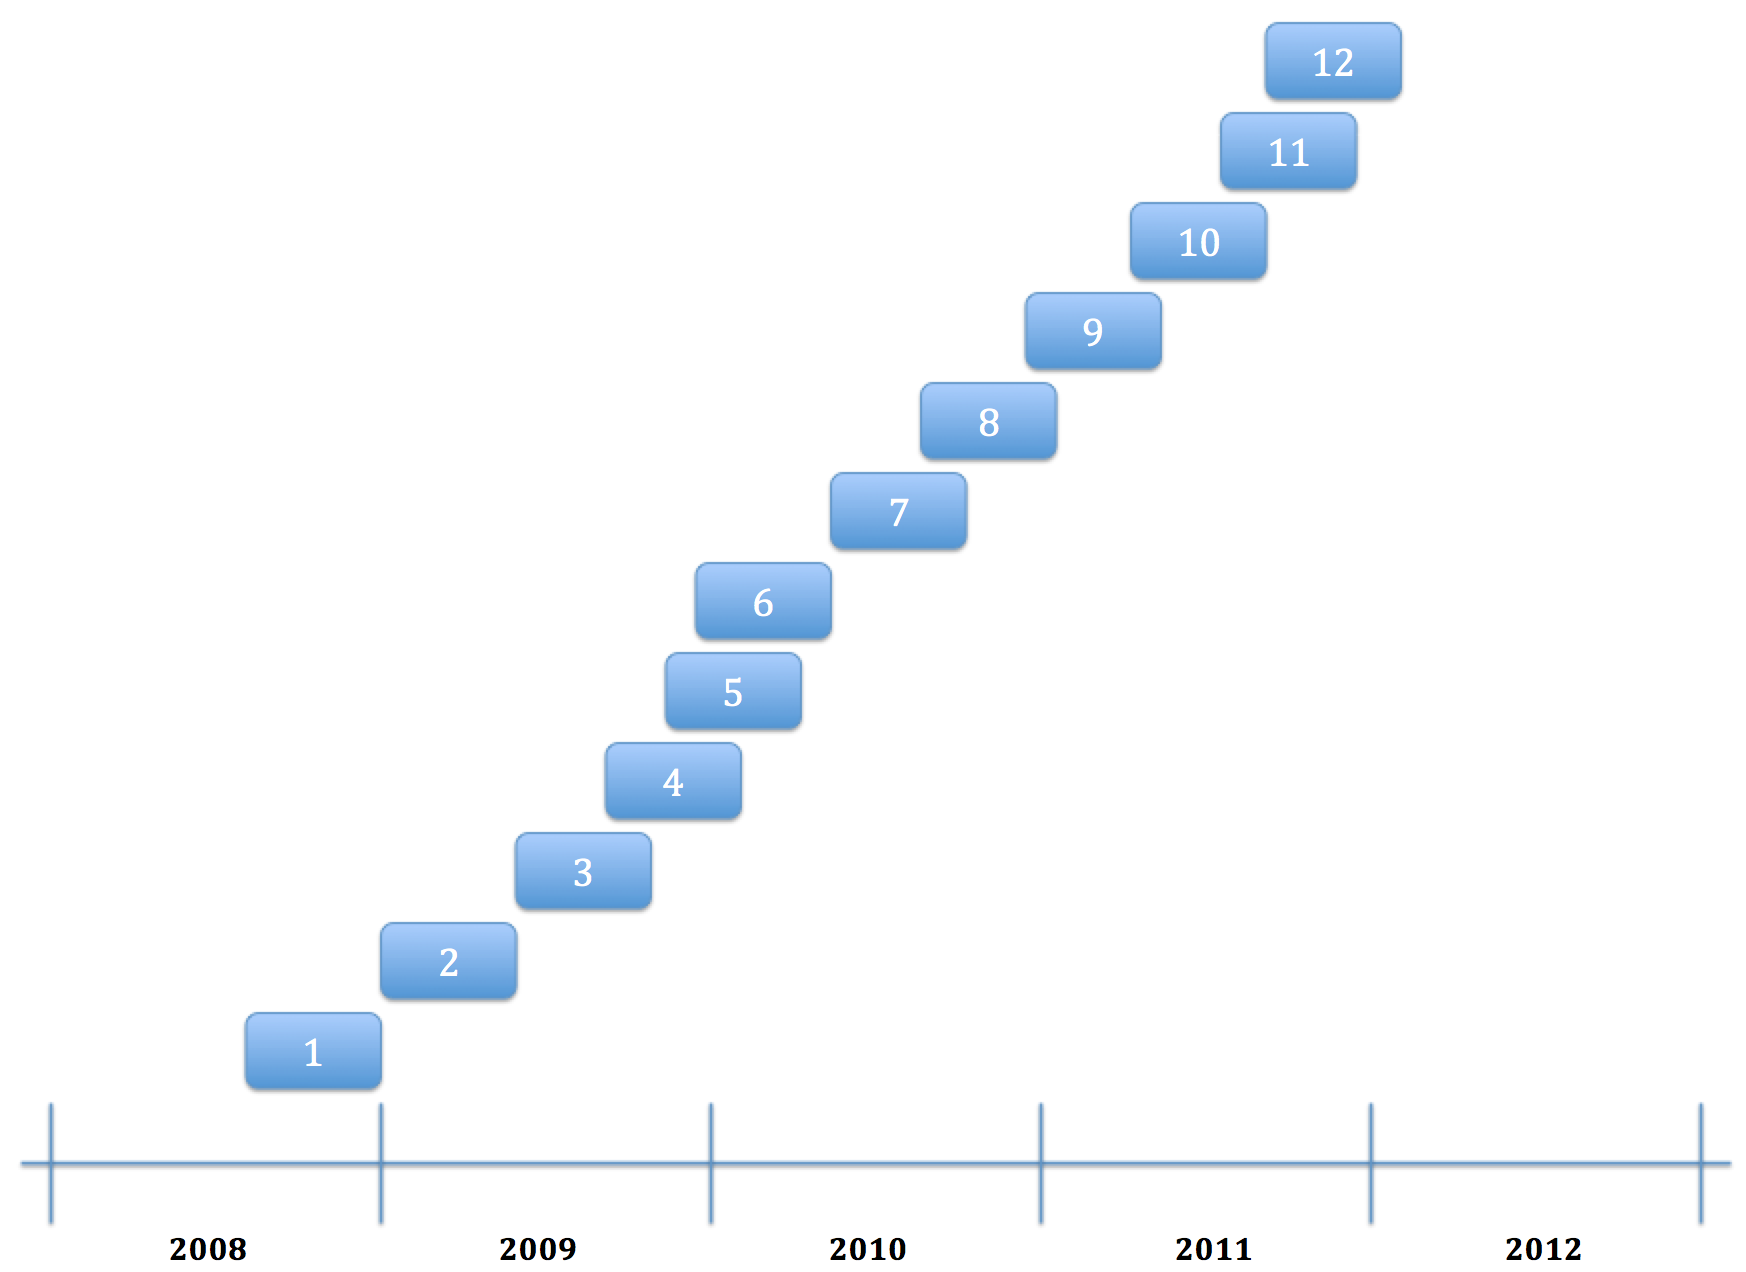
\includegraphics[trim = 8mm 0mm 0mm 0mm,width=160mm]{images/project_releases}
\caption{Main project releases in Omega.}
\label{releases}
\end{figure}

The initial project execution model consisted of six phases involving different personnel. The planned project execution was as follow: Starting of the project was a general requirements phase where also potential impacts were assessed, here both business resources and architectures were present. Following the general overview phase was a requirements analysis phase, again with both business and architecture resources. After these more general phases the solution description was worked on. The solution description was the main responsibility of the architecture unit, but business resources, developers, test resources and the heads of delivery were included. Going into the construction and approval phases all resources were collaborating to get continuous deliveries finished for production. In the production phase the main responsibility was put on the heads of delivery, but business and line resources were also present throughout the whole process, and architects, developers and testers were included in parts of the phase. The whole project execution model can be seen in figure \ref{project_execution}.

\begin{figure}
\centering
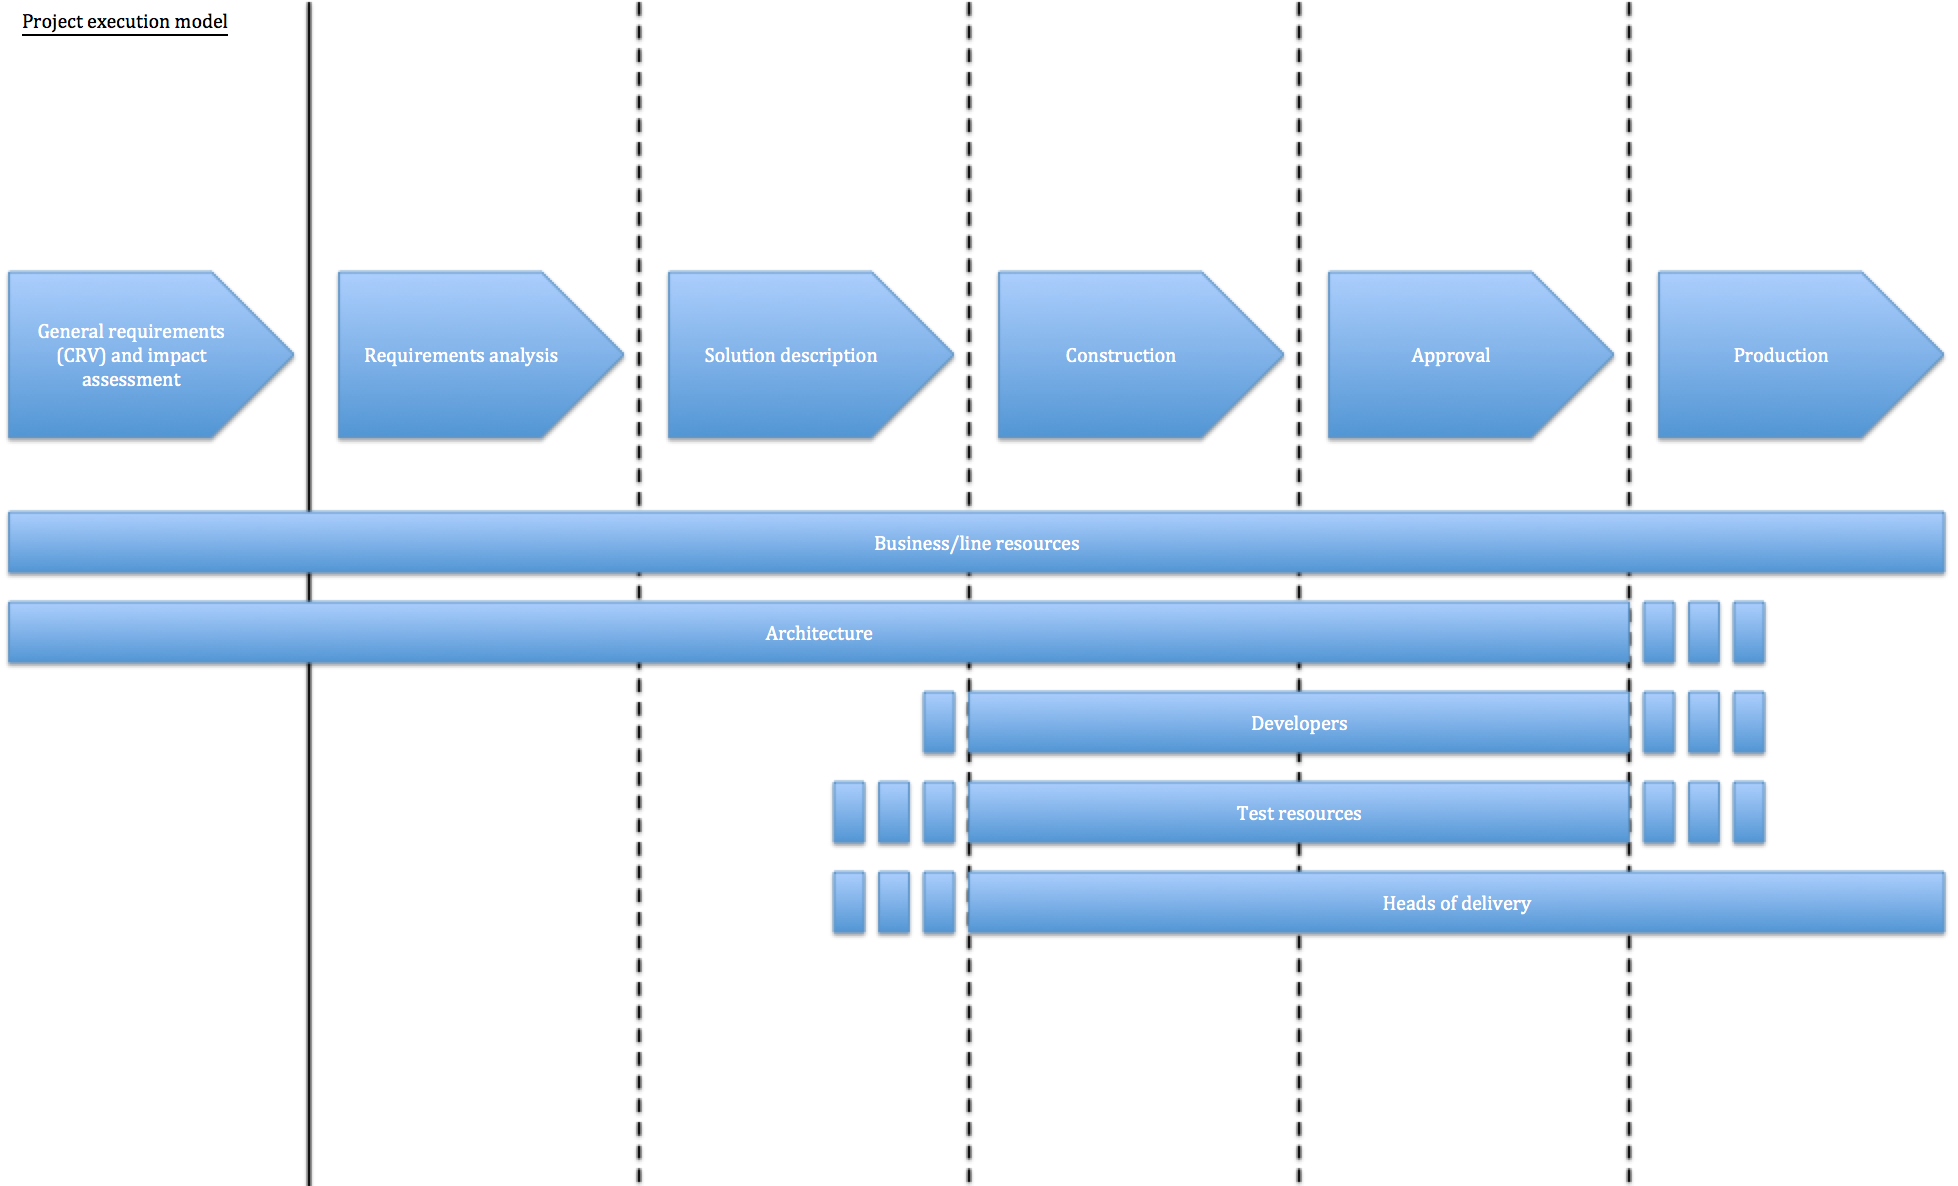
\includegraphics[angle=90, trim = 0mm 0mm 20mm 0mm,width=160mm, height=230mm]{images/execution_model.png}
\caption{Project execution model.}
\label{project_execution}
\end{figure}

The project was organised with a ``project director'' at the top of the hierarchy mainly focusing on external relations. Underneath the project director there was a ``project manager'' responsible for operations. Omega also had four sub-projects with one ``sub-project manager'' each. These sub-projects were architecture, business, development and test, and are further described below. There were also a ``controller'' (or ``secretary'') present for administrative reasons. As can be seen from figure \ref{omega} the project used a matrix structure where the business and development sub-projects were both closely linked to the test and architecture sub-projects.

%TODO: Endre Alfa til Alpha
\begin{figure}[H]
\centering
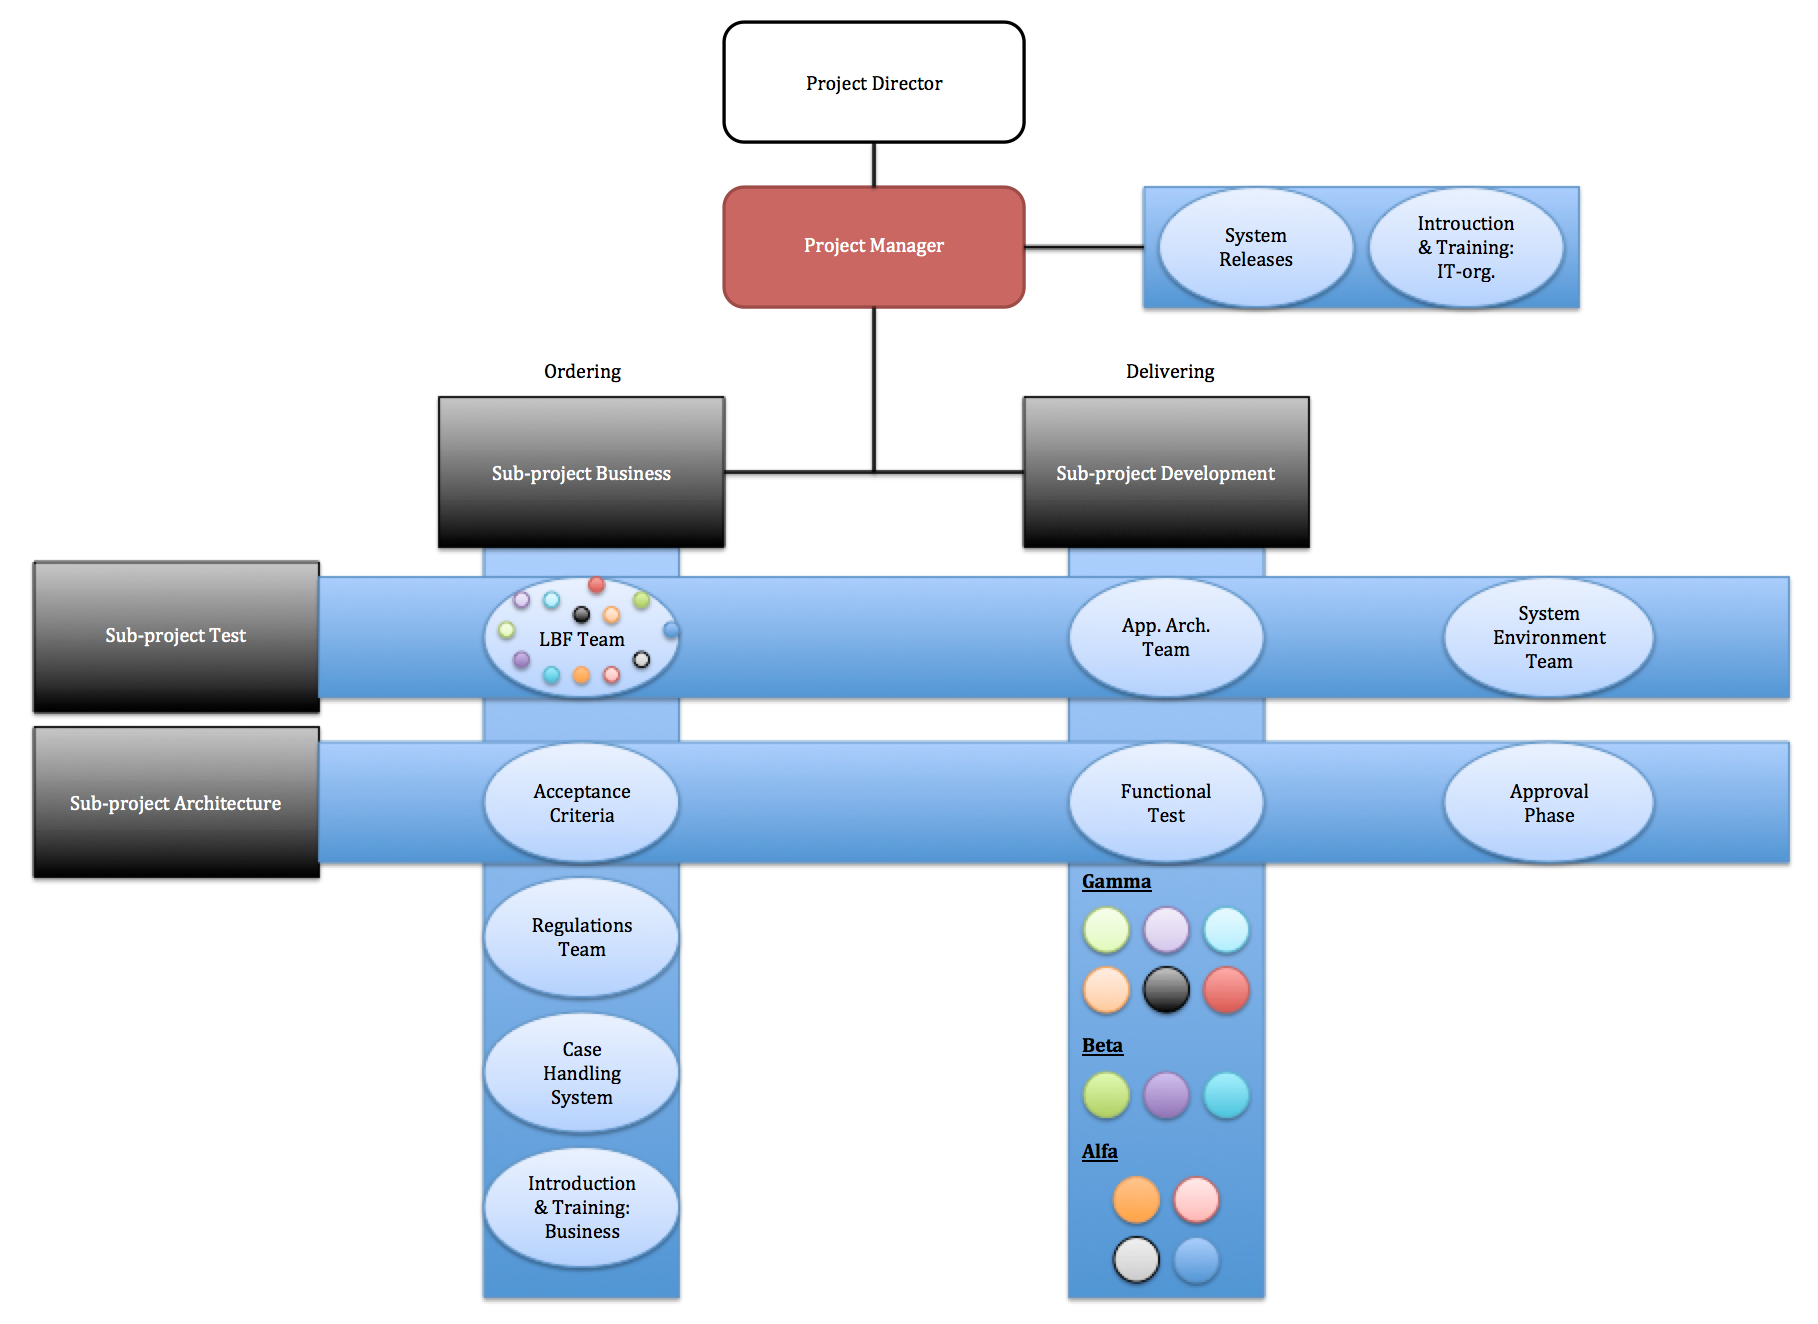
\includegraphics[trim = 0mm 0mm 0mm 0mm,width=150mm]{images/omega_organisation.png}
\caption{Omega-project's organisation.}
\label{omega}
\end{figure}

\begin{itemize}
   \item \textbf{Architecture:} Architects were in general responsible for the overall architecture of the project, but more specifically focused on solution description. They were also important in dealing with dependencies in Omega, and continuously updated a dependency map. The sub-project had both head architects and technical architects located on a team level.
   \item \textbf{Business:} The business and line resources were present in the whole execution of the project (as can be seen from figure \ref{project_execution}). The responsibility of the business sub-project was categorise needs and requirements, and then defining these into epics and user stories in a product backlog. In this sub-project there was a product owner team, but also other business and line resources (approximately 30 members at a peak period). Both functional and technical architects from the Scrum teams were also involved in the business sub-project.
   \item \textbf{Development:} The construction sub-project was further divided into three sub-projects led by Alpha, Beta and Gamma. The Gamma organisation had at most six development teams involved with both their own personnel and external consultants hired in from five different consulting companies. Alpha had at most four teams, while Beta had a maximum of three development teams. All 13 component teams worked corresponding to the Scrum methodology and delivered on a common demo day at the end of every three-week sprint iteration. There was also a system environment team present which was in charge of development and test environments. All roles of the Scrum teams are outlined in table \ref{trpist}.
   \item \textbf{Test:} The test sub-project had responsibility for all the testing of the project and the providing of deliverables from the development teams. Hence, they were important for quality assurance. The sub-project included a test leader, as well as test personnel from the development teams.
\end{itemize}

The main focus of this thesis has been on development of the system. The development iterations had four phases: ``analysis of need'', ``solution description'', ``construction'' and ``approval''. These are further described below. The development process can be seen in figure \ref{initial_development_process}.

\begin{itemize}
   \item \textbf{Analysis of need:} Starting of each development release was an analysis phase. Here the focus was on functionality to be included in the coming release, and identifying and working out user stories. The product owner was involved in this process and was, e.g., responsible for prioritising the product backlog.
   \item \textbf{Solution description:} After identifying and working out general user stories in the ``analysis of need'' phase the user stories were further developed and made more comprehensive in the ``solution description'' phase. These user stories were also assigned to epics, and further estimated in approximate work-hours to completion before being assigned to different Scrum teams. Design and architectural choices were also determined in this phase.
   \item \textbf{Construction:} The construction phase typically consisted of five to seven sprint iterations per main development release. Here all development was carried out, and all work was functionally tested.
   \item \textbf{Approval:} In the last phase of each development release the delivered functionality was tested, both formal and non-formal functional testing. This was done to assure both the internal and external interfaces were working as expected.
\end{itemize}

\begin{figure}
\centering
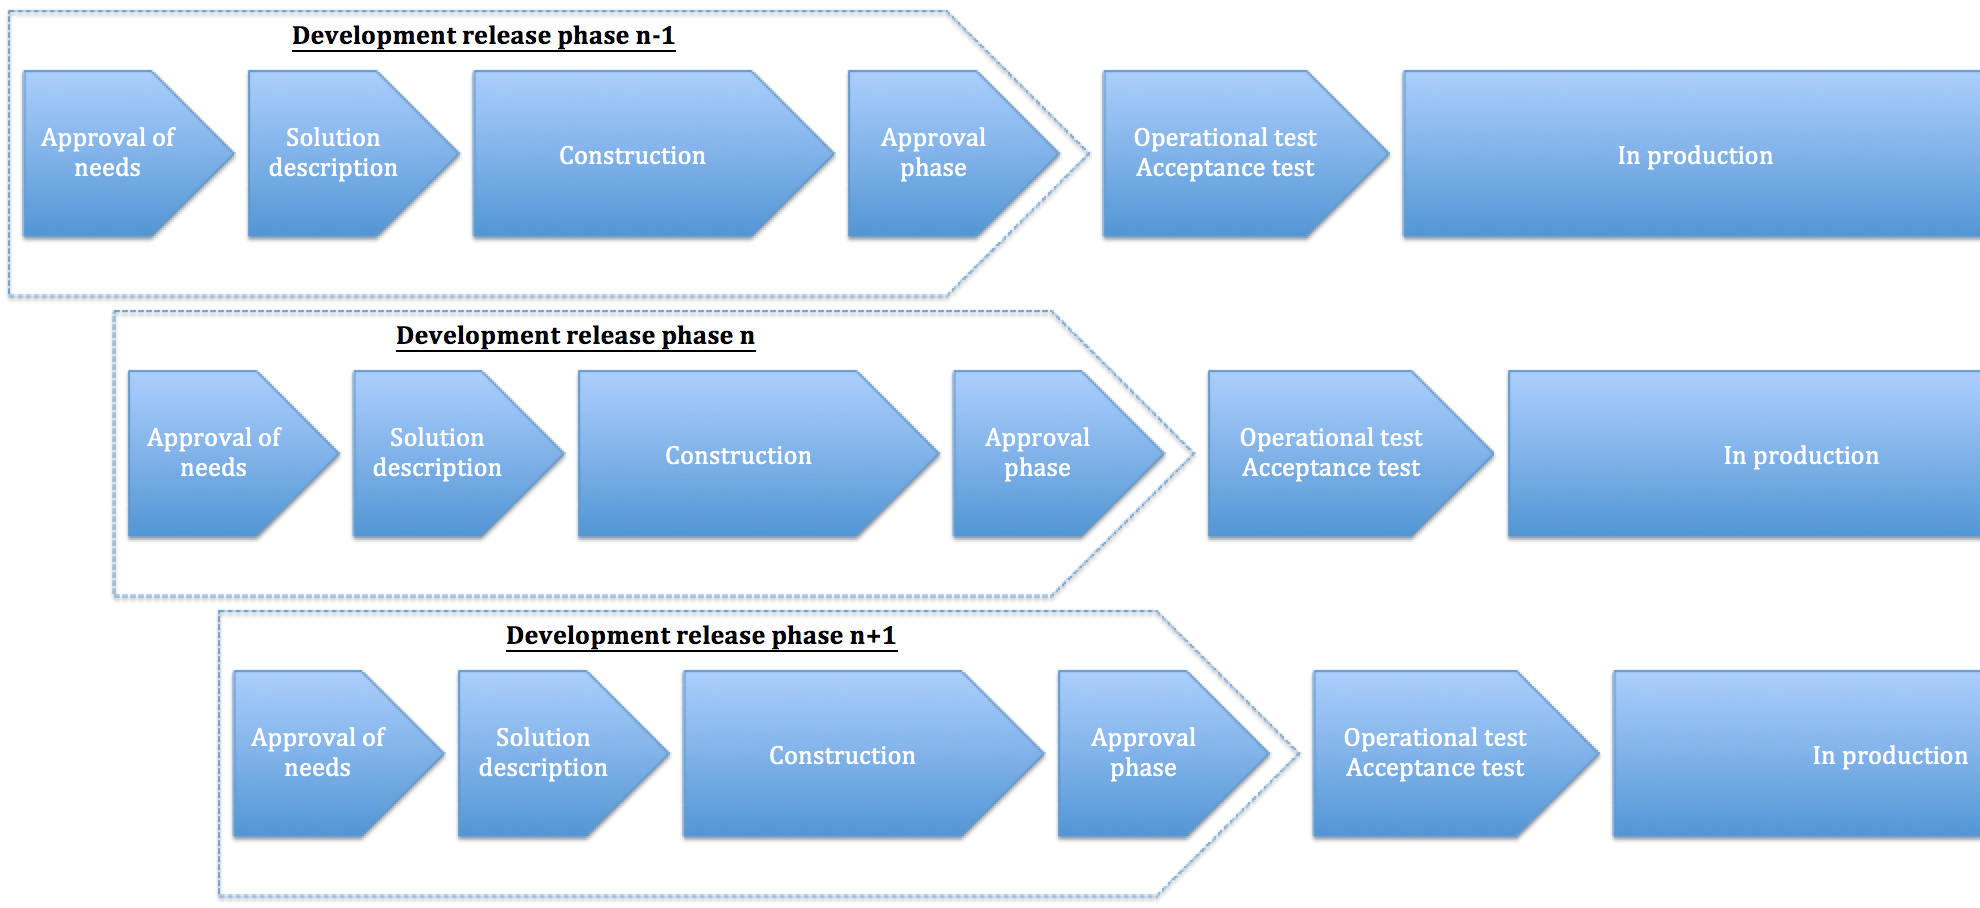
\includegraphics[angle=90, trim = 0mm 0mm 20mm 0mm,width=160mm, height=230mm]{images/initial_development_process}
\caption{Initial development process.}
\label{initial_development_process}
\end{figure}

The development phase consisted primarily of several Scrum teams typically involving eight to nine members each. The roles in the different Scrum teams are further outlined in table \ref{trpist}. It is however important to remember that all members were somewhat cross-functional in the project. This means that a tester could for example have been 60\% tester, 30\% developer and 10\% designer, and a Scrum master could have been 50\% leader, 30\% architect and 20\% developer. 

%TODO: Ta en kikk på roller en gang til
\begin{table}[H]
\begin{center}
    \begin{tabular}{| p{4cm} | p{8cm} |}
    \hline
    \textbf{Role} & \textbf{Description of role} \\ \hline
    Scrum master & The Scrum master facilitated all meetings such as the daily stand-up, demo presentations, retrospectives and iteration planning. Some teams rotated the role, while others had a fixed Scrum master. \\ \hline
    Functional architect & The functional architect was typically working 50\% with analysis and design, and 50\% as a developer. \\ \hline
    Technical architect & About half of the time went towards technical design, while the other half usually was spent developing. \\ \hline
    Tester & The person with the title ``tester'' was not responsible for doing all the testing, but was rather responsible for the tests being conducted. He was also in charge of writing and delivering test criteria to the sub-project test. The tests at the team level was unit tests, integration tests, system tests and system integration tests. Some of the teams did not have fixed testers, but rotated the role somewhat, e.g., at Beta. \\ \hline
    Developer & Each team had a mixture of four to five junior and senior developers. \\ \hline
    \end{tabular}
    \caption{Team roles present in Scrum teams.}
    \label{trpist}
\end{center}
\end{table}

\begin{table}[H]
\begin{adjustwidth}{-1.15cm}{}
%\begin{center}
\begin{tabular}{ | p{2.7cm} | p{5cm} | p{9cm} | }
	\hline
	\textbf{Dimension} & \textbf{Attribute} & \textbf{} \\ \hline
	\multirow{10}{*}{Compositional} & Number & There was a maximum of 13 development teams (but also other teams involved such as project management) \\ \cline{2-3}
 	& Size & Approximately 175 members involved in the MTS \\ \cline{2-3}
 	& Boundary status & Multiple organisations (mer?) \\ \cline{2-3}
 	& Organisational diversity & There were in total five organisations taking part in the project, though three of these were the main organisations with the most members allocated to the project \\ \cline{2-3}
	& Proportional membership & Alpha had four development teams (31\%), Beta had three teams (23\%) and Gamma had six component teams (46\%) \\ \cline{2-3}
	& Functional diversity & Somewhat high degree of heterogeneity in core purposes and missions of teams \\ \cline{2-3}
	& Geographic dispersion & The teams were co-located in the same open-plan office space \\ \cline{2-3}
	& Cultural diversity & Low degree \\ \cline{2-3}
	& Motive structure & High degree (?) \\ \cline{2-3}
	& Temporal orientation & High? \\ \cline{2-3}
\hline
	\multirow{5}{*}{Linkage} & Interdependence & ? \\ \cline{2-3}
 	& Hierarchical arrangement & Development teams located at the same level in the hierarchical arrangement \\ \cline{2-3}
 	& Power distribution & The development teams had an even power distribution \\ \cline{2-3}
	& Communication structure: Network & Both informal and formal communication patterns \\ \cline{2-3}
	& Communication structure: Modality & Mainly face-to-face communication \\ \cline{2-3}
\hline
	\multirow{6}{*}{Developmental} & Genesis & Appointed \\ \cline{2-3}
 	& Direction of development & ? \\ \cline{2-3}
	& Tenure & Approximately four years \\ \cline{2-3}
	& Stage & Finished \\ \cline{2-3}
	& Transformation of system composition: Membership constancy & Some fluidity depending on need throughout the Omega-project \\ \cline{2-3}
	& Transformation of system composition: Linkage constancy & Some communication lines and arenas were fluid, changing base on a need basis, while others were constant through the whole project \\ \cline{2-3}
	\hline
\end{tabular}
\caption{Overview of the Omega-project in a MTS fashion}
\label{ootopiamf}
%\end{center}
\end{adjustwidth}
\end{table}

%\begin{table}[H]
\begin{center}
    \begin{longtable}{| p{6cm} | p{9cm} |}

    \hline \textbf{Coordination mechanism} & \textbf{Description of mechanism} \\ \hline
    \endfirsthead

    \multicolumn{2}{c}%
{{\bfseries \tablename\ \thetable{} -- continued from previous page}} \\ \hline
    \textbf{Coordination mechanism} & \textbf{Description of mechanism} \\ \hline
    \endhead

    \multicolumn{2}{|r|}{{Continued on the next page\ldots}} \\ \hline
    \endfoot

   \endlastfoot

    Metascrum & A meeting similar to Scrum of Scrums but with less details which was held twice per week. Attending the metascrum was the project leaders and all the sub-project leaders from test, architecture, business and development. A ``technical metascrum'' was tried, but was shortly shut down after initiation. \\ \hline
    Planning day & The planning day was a form of kick-off for each sprint iteration where the project members met up with the project owner. The planning day was performed on three levels: project, organisation (Alpha, Beta and Gamma) and team. A rough sketch of the focus areas and work to be performed in the coming sprint was presented with a distribution towards each of the three organisations by the project owner. After this the organisations distributed the work on their respective teams, and lastly the teams got together separately and worked out a contract with estimated work to be performed which was delivered to the project owner team. Before the planning day commenced the developers also had a ``developer forum'' where development-oriented information and discussion was carried out. This was however held on an organisation basis, and not across the three organisations. \\ \hline
    Demo & Demo presentations were held by all Scrum teams at the end of each sprint iteration where everyone could attend. Each team was allocated approximately 10 minutes. There were also larger demo presentations for the project owner when a new release was finished. Some teams in addition started performing smaller demo sessions within the iterations to get rapid feedback. \\ \hline
    Pre-planning day & Before the ``planning day'' was carried out a pre-planning day was performed. Here typically different types of architects (especially functional architects) and the project owner (as well as some other members of the project owner's team) met to create a rough classification and allocation of work to the different Scrum teams for the coming sprint iteration. The allocated work was listed in a prioritised manner. \\ \hline
    Dependency meeting & A meeting held between all Scrum masters from the Alpha, Beta and Gamma teams. This meeting was held on the ``Planning day'' where the focus was on discovering dependencies across Scrum teams. However, these meetings faded away early on because of the dependencies being discovered and handled elsewhere. \\ \hline
    Solution description / ``Master plan'' & At the start of the Omega-project a larger solution description phase was performed involving a lot of architects (as can be seen from figure \ref{project_execution}). This lead to a ``master plan'' for the project and was documented in an issue tracker program called Jira. The ``master plan'' was continuously altered throughout the course of the development phase as outlined in figure \ref{initial_development_process}. In the solution description meetings important aspects were discussed such as coordination across organisations and management of activities. An example of what came out of these meetings was a dependency map of the whole Omega-project, which was in constant change. Part of the solution description meetings were also negotiation and estimation meetings which were important for the contract for each release. \\ \hline
    Jira and Wiki/Confluence & Different programs and forums were used for documentation and tracking within the project. In Jira all user stories and epics were located, and different information about the project and current sprint iteration could be seen on different levels, such as project and team level. The dependency map for the whole Omega-project was also located in Jira. Confluence was the main program used as a wiki. Here solution descriptions, team routines, routines across teams, system documentation, check lists, retrospectives, architectural guidelines, functional test etc. were all located. \\ \hline
    Open-space & An arena held on a voluntary and need basis, which was used for exchanging experiences. Only used during a few of the releases. Participants suggested the topics beforehand, leading to agendas for open-space sessions. \\ \hline
    Jabber & Jabber was introduced as an instant messaging service in the Omega-project after being identified as something needed in one of the Open-space sessions. Project members could ask both formal questions, e.g., technical questions, and informal questions or activities, e.g., wine lotteries. \\ \hline
    Lunch seminars & Kind of similar to the ``open-space'' sessions. Typically two to three topics were held by project-personnel on relevant and interesting topics, often regarding themes correlated to the current situation of the project. As with the ``open-space'' session these seminars were also held on a certain period of the project before fading away. \\ \hline
    Front-end meeting & The front-end developers worked with a complex framework called Flex. Because of this a lot of coordination had to be handled between teams working with this framework from all organisations. Therefore, front-end meetings where held were typically the most prominent Flex-developers were present. \\ \hline
    Technical architecture forum & At the technical architecture forum all technical architects met up to discuss what was to be done in the coding base to prevent coordination issues. These meetings were slowly fading away because the need was covered in other arenas. \\ \hline
    Architecture council & At these gatherings an architecture council listened to all team architects present their respective team's tasks for each sprint iteration. \\ \hline
    Business meeting & The business part of the Omega-project was coordinated through meetings where the business architects from Alpha, Beta and Gamma met up with the business unit from the project owner. Here the sprint iteration queue, and the current status of the project and sprint was presented. This meeting was held around one time each week or every other week. \\ \hline
    Bug-board discussion & The quality assurance unit with its testers had frequent meetings around bug-boards, especially after new releases and around acceptance testing. In the period after a new release these meetings were often held on a daily basis. Here all the bugs were gone through and allocated to the responsible Scrum team in either Alpha, Beta or Gamma. \\ \hline
    
    \caption{Coordination mechanisms used across the whole Omega-project.}
    \label{cmuatwo} 
    \end{longtable}
\end{center}
%\end{table}

\begin{center}
    \begin{longtable}{| p{6cm} | p{9cm} |}

    \hline \textbf{Coordination mechanism} & \textbf{Description of mechanism} \\ \hline
    \endfirsthead

    \multicolumn{2}{c}%
{{\bfseries \tablename\ \thetable{} -- continued from previous page}} \\ \hline
    \textbf{Coordination mechanism} & \textbf{Description of mechanism} \\ \hline
    \endhead

    \multicolumn{2}{|r|}{{Continued on the next page\ldots}} \\ \hline
    \endfoot

   \endlastfoot

    Scrum of Scrums (SoS) & Scrum of Scrums were meetings held by all organisations (Alpha, Beta and Gamma) ranging from two to three times per week. In these meetings all Scrum masters from the corresponding organisation, as well as project management (project leader, test leader, head technical architect, head functional architect, business leader and development leader). The main goal of the SoSs was to identify and handle obstacles. There were also held a few SoS meetings across organisations to handle potential changes to the contracts. \\ \hline
    Technical corner & The ``technical corner'' was a meeting Beta had in an early stage of the project. It was held on Fridays for about 1-1,5 hour. Here team architects presented important themes for the Beta-members. After a while it was shut down because of lack of interest and topics. \\ \hline
    Experience forum & The experience forum was an arena established in the Alpha-organisation for exchanging experiences. Here Scrum masters and the development manager met to discuss topics such as retrospectives, the planning day, and how work was performed by the Alpha-organisation's Scrum teams. It could be seen as a coaching-session with exchange of ideas and thoughts. \\ \hline
    Retrospective & Retrospectives were used on several levels in the project. All of the organisations used it on a pure Scrum team level, but some also used it on both the solution description personnel and in the project management team. The retrospectives for each Scrum team were held after the demo on Fridays. Here negative and positive information and aspects were brought forward and documented in Confluence. A few ``global retrospectives'' were also tested but swiftly faded away. \\ \hline
    Technical and functional architecture meetings & Both technical and functional architects had separate meetings within the different organisations. These meetings were typically short and held on a weekly or biweekly basis. The meetings were as mentioned brief and were primarily used for status updates, and keeping the technical and functional managers up-to-date to make the cross-coordination meetings with the other organisations easier and more precise. \\ \hline
    Supplier meeting & At Alpha a supplier meeting was held by the project leader for all Alpha-members. The project leader contributed with practical information regarding the project. In these meetings different members held presentation on different topics such as clean code, test driven development and project guidelines to keep the technical level up to scratch on the personnel. \\ \hline
    Meeting about queue & Alpha also had a meeting regarding ``what was next in the queue?'', ``what is the next delivery?'', ``what is the status on current user stories?'' and ``what is it that we feel is needed to drive the queue forward?''. In these meetings was held with the functional architect, development manager and product owner from Gamma. \\ \hline

    \caption{Coordination mechanisms used across teams within the specific organisations (Alpha, Beta and Gamma) in the Omega-project.}
    \label{cmuasito}
    \end{longtable}
\end{center}

\begin{center}
    \begin{longtable}{| p{6cm} | p{9cm} |}
   
    \hline \textbf{Mechanism/Aspect} & \textbf{Description} \\ \hline
    \endfirsthead

    \multicolumn{2}{c}%
{{\bfseries \tablename\ \thetable{} -- continued from previous page}} \\ \hline
    \textbf{Coordination mechanism} & \textbf{Description of mechanism} \\ \hline
    \endhead

    \multicolumn{2}{|r|}{{Continued on the next page\ldots}} \\ \hline
    \endfoot

   \endlastfoot 

    Stand-up & Daily stand-ups were used on all Scrum teams in the project. Here obstacles, progression and possible needs were voiced around the Scrum-boards. Introduced by Gamma was also the way of organising the stand-up meeting such that they were held on different timeslots. This made it possible for members to attend several stand-ups if necessary. \\ \hline
    Board discussion & An important aspect for coordination, discussion and status updates in the project was the frequent use of whiteboards. The stand-up meetings were for instance held around these boards, and on these boards the workload for each sprint iteration was put up and updated as the sprint moved along. The backside of the boards were left open to carry out informal discussion when needed. \\ \hline
    Co-location & One of the biggest impacts on the project, and coordination, collaboration and communication within the project was the radical co-location. This co-location came at any early stage (with the introduction of Alpha and Beta in Omega) in the project where all teams, as well as project management, were located in an open-plan office space at the same floor. \\ \hline
    Project management in same location & In both Alpha and Beta management by ``walking around, talking around'' was brought up. Because the project management was located in the same office space as the other project teams it was easy for them to keep track and manage by just being present. With management being close by it was, e.g., possible for development managers to have informal communication with each Scrum master every day, making sure they were up-to-date on the progress. This lead to easier decision making and problem handling for the project management team. Another important and positive factor was that decision making could be taken rapidly through more informal arenas, as teams could address project management at once without having to book formal meetings every time a decision had to be made. \\ \hline
    Informal communication & Another important impact on the coordination and general information sharing was the extensive use of informal communication. These communication arenas seemed to be very important in the agile mindset because of the pressure on delivering within a short period of time. With the use of informal communication arenas decisions could be made faster than using formal arenas such as having to book meetings where, e.g., timeslots had to match for participants. As the project progressed the informal communication arenas were more and more present, often replacing some of the formal communication arenas. \\ \hline
    Joint coffee break & An informal communication arena that was present throughout the Omega-project was the ongoing discussion around the coffee machine area. There were even joint coffee breaks at 2PM every day. These informal meetings saw a growth as the project moved along. \\ \hline
    Pair-programming & Pair-programming was introduced by Beta and adopted by some of the other organisations. Often the pairs constituted of one senior and one junior developer. The main reasons for using pair-programming was to achieve a higher standard on the coding, increase knowledge (especially of junior developers) and to build better relationships and trust within teams. Pair-programming was also tested across teams, but was not deemed successful. \\ \hline
    Trust & Another important aspect of the project was trust, both within and across organisations, but also between the organisations (Alpha, Beta and Gamma) and the product owner. Trust was increased through several ways, e.g., social gatherings, co-location and a general openness culture. With the increase in trust between the different project-members there was an increase in informal communication arenas, and a decrease in formal ones, leading to more rapid decision making, in line with the agile mindset. \\ \hline
    Rotation of team members & At Beta some rotation of members across the Scrum teams happened. This was mainly to spread competence and knowledge across teams to make them more ``all round teams'' able to handle different types of work. There were also a few rotations because of personal chemistry. \\ \hline
    Rotation of team placement & Another decision made by Beta and Gamma was to change location within the office space of some teams. This was a deliberate move by the project management to achieve better collaboration and communication, especially on the informal level, between teams working on similar parts of the project. \\ \hline
    Alpha/Beta-personnel placed in Gamma teams & An aspect that might have been important both for trust and the informal communication was that both Alpha and Beta members were located in Gamma teams. This probably made it easier to get informal communication going at an early stage of the Omega-project because some members knew each other across the organisations already. \\ \hline
    Continuous planning and change & Self-organising was present at different levels in Omega such as team, organisation and project level. At the team level the teams changed their ways as the project moved along introducing new and removing old aspects, e.g., moving from pair-programming to individual programming when knowledge increased. At both the organisational level and the project level different communication arenas were changed on a need-basis. This had mainly to do with the respective arenas being covered elsewhere, e.g., through informal communication. Another part of the project where continuous planning and change was present was within the dependency mapping and solution description. \\ \hline
    3-level hierarchy from product owner & Mentioned by Gamma was the way the product owner was organised within the project. At the top of the food change the main product owner sat, then three representatives from the product owner were located at Alpha, Beta and Gamma, and at the bottom of the hierarchy the product owner had functional experts and architects inside or close to the teams. This led to easier decision making as the representatives further down the hierarchy could answer on the behalf of the product owner, or at least knew who to ask for the answer increasing the pace of development and problem solving. \\ \hline

    \caption{Other coordination mechanisms and important aspects.}
    \label{ocmaia}
    \end{longtable}
\end{center}

%Trust
%A teamwork model for understanding an agile team: A case study of a Scrum project
%http://www.uio.no/studier/emner/matnat/ifi/INF5181/h14/artikler-teamarbeid/salas_etal_2005_is_there_a_big_five_in_teamwork---copy.pdf

% http://ieeexplore.ieee.org/xpl/articleDetails.jsp?arnumber=5287007 Har definisjon av trust og andre aspekter
% http://ieeexplore.ieee.org/xpl/articleDetails.jsp?arnumber=926814&contentType=Conference+Publications
% S. P. Shapiro, "The Social Control of Impersonal Trust", American J. Sociology, vol. 93, no. 3, pp. 623-658, 1987
% J. M. Wilson , S. G. Straus and W. J. McEvily, "All In Due Time: The Development of Trust in Computer-Mediated and Face-to-Face Groups", Organizational Behavior and Human Decision Processes, vol. 99, pp. 16-33, 2006

% http://onlinelibrary.wiley.com/doi/10.1111/j.1467-8608.2008.00517.x/full
% Kassicieh, S.K., Walsh, S.T., Cummings, J.C., McWhorter, P.J., Romig, A.D. and Williams, W.D. 2002. ‘Factors differentiating the commercialization of disruptive and sustaining technologies. IEEE Transactions on Engineering Management, 49:4, 375–387. 
% Stuart, T.E. 1998. ‘Network positions and propensities to collaborate: an investigation of strategic alliance formation in a high-technology industry. Administrative Science Quarterly, 43:3, 668–698. 
% Gulati, R. 1999. ‘Network location and learning: the influence of network resources and firm capabilities on alliance formation. Strategic Management Journal, 20:5, 397–420. 
% Ahuja, G. 2000. ‘Collaboration networks, structural holes and innovation: a longitudinal study. Administrative Science Quarterly, 45:3, 425–455. 
% McEvily, B. and Marcus, A. 2005. ‘Embedded ties and the acquisition of competitive capabilities. Strategic Management Journal, 26:11, 1033–1055. 

